%File: aaai2027-unified-supp.tex
%
% AAAI 2027 SUPPLEMENTARY MATERIAL
% To switch between anonymous submission and camera-ready versions,
% simply change the next line:
%
% For ANONYMOUS SUBMISSION: uncomment the next line
\def\aaaianonymous{true}
%
% For CAMERA-READY VERSION: comment out or delete the next line
% \def\aaaianonymous{true}
%
%%%%%%%%%%%%%%%%%%%%%%%%%%%%%%%%%%%%%%%%%%%%%%%%%%%%%%%%%%%%%%%%%%%%%%%
%
% NOTE (2026-07-20): this file documents the method and BOTH experimental venues of the main
% paper. Section A specifies the METHOD. Section B is the SIMULATION venue
% (residual RL trained directly against the DexMimicGen/LIBERO simulators); Section C
% is the REAL-ROBOT venue (the shared residual objective trained inside a learned
% dynamics model). It remains a protocol-forward draft: every quantity here is
% either verified from the actual pipeline or marked \todo{}. The main paper carries
% the compact headline tables; this supplement reserves reader-facing per-seed and
% paired-result sections, which remain TODO while the simulation inventory is reconciled
% and the real-robot evaluation is pending. The simulation hyperparameters in
% Section B.3 were extracted from the trainer/config source
% (resfit/rl_finetuning/); the naming convention that encodes them in the run
% scripts is: as005 = action_scale 0.05, bc01 = demo_bc_coef 0.1,
% hiqlv512 = goal-conditioned value width 512, sg15 = subgoal_way_steps 15.
%
%%%%%%%%%%%%%%%%%%%%%%%%%%%%%%%%%%%%%%%%%%%%%%%%%%%%%%%%%%%%%%%%%%%%%%%

\documentclass[letterpaper]{article} % DO NOT CHANGE THIS

% Conditional package loading based on version
\ifdefined\aaaianonymous
    \usepackage[submission]{aaai2027}  % Anonymous submission version
\else
    \usepackage{aaai2027}              % Camera-ready version
\fi

% aaai2027.sty loads the required newtxtext, helvet, and courier fonts.
\usepackage[hyphens]{url}  % DO NOT CHANGE THIS
\usepackage{graphicx} % DO NOT CHANGE THIS
\urlstyle{rm} % DO NOT CHANGE THIS
\def\UrlFont{\rm}  % DO NOT CHANGE THIS
\usepackage{natbib}  % DO NOT CHANGE THIS AND DO NOT ADD ANY OPTIONS TO IT
\usepackage{caption} % DO NOT CHANGE THIS AND DO NOT ADD ANY OPTIONS TO IT
\frenchspacing  % DO NOT CHANGE THIS

\usepackage{amsmath}
\usepackage{amssymb}
\usepackage{booktabs}

\pdfinfo{
/TemplateVersion (2027.1)
}

\setcounter{secnumdepth}{0} %May be changed to 1 or 2 if section numbers are desired.

% draft-only helper (remove before submission), matching main.tex
\newcommand{\todo}[1]{\textbf{[TODO: #1]}}
\newcounter{algorithm}

% Title - conditionally set based on version
\ifdefined\aaaianonymous
    \title{SHORE-RL: Shortening Effective Horizon for Long-Horizon Residual\\
    Reinforcement Learning\\
    \vspace{0.5em}\large Supplementary Material}
\else
    \title{SHORE-RL: Shortening Effective Horizon for Long-Horizon Residual\\
    Reinforcement Learning\\
    \vspace{0.5em}\large Supplementary Material}
\fi

% Author and affiliation information
\ifdefined\aaaianonymous
\author{
    Anonymous Submission
}
\affiliations{
    % Leave affiliations empty for anonymous submission
}
\else
\author{
    Anonymous Submission
}
\affiliations{
}
\fi

\begin{document}

\maketitle

\begin{abstract}
This supplement documents the SHORE-RL objective and the implementation details
currently recoverable from the retained code and artifacts, followed by the simulation
and real-robot experimental protocols. The two venues share
the same residual policy parameterization and actor--critic update, while instantiating
different transition collectors, reward sources, and replay samplers. We additionally
document the ablation design, available run provenance, qualitative dynamics-model
evidence, and the physical-robot evaluation controls needed to interpret the
main-paper results. Unavailable validation results and provenance fields are marked
explicitly rather than inferred.
\end{abstract}

% Supplementary Content Starts Here

\section{A\quad Method and Implementation Details}

The main paper introduces the residual controller, self-derived waypoint, and two
dense-reward choices. Here we give the method-level optimization objective and the venue-parameterized update of
Algorithm~\ref{alg:shore}, in the notation the two venues reuse. Shared architectural
settings and the simulation defaults are collected in Table~\ref{tab:sharedhp};
venue-specific numbers and overrides appear in Section~B.3 and Section~C.5.

\subsection{A.1\quad Residual Coordinates and Decision Time Scale}

We write the navigator state as
$e_t=\operatorname{Std}([\psi_b(o_t);q_t])$, where $\psi_b$ is the
frozen base-policy feature and $q_t$ is proprioception; implementation tables
occasionally abbreviate this feature as $s_t$. The residual actor and critic do
\emph{not} use $\psi_b$: they share a trainable multi-view image encoder,
distinct from $\psi_b$ and updated only through the critic loss
(Section~A.4). Both additionally read proprioception and the waypoint $z_t$;
the actor also receives the base action $a_t^b$, whereas the critic conditions
on the projected combined action $a_t$ and does not take $a_t^b$ as a separate
input.

Let $f_\theta$ denote the actor's pre-squash output. The deterministic scaled
residual mean and projected normalized command are
\[
\begin{aligned}
\mu_\theta(o_t,a_t^b,z_t)
&=s_a\tanh\!\big(f_\theta(o_t,a_t^b,z_t)\big),\\
a_t&=\Pi_{\mathcal A}(a_t^b+\delta_t),
\end{aligned}
\]
where collection samples $\delta_t$ around $\mu_\theta$ using the exploration
rule in Section~A.4, while evaluation uses $\delta_t=\mu_\theta$. The same
projected normalized action $a_t$ is passed to the collector (and to the
dynamics model in imagination) and stored in replay. The environment may
subsequently convert this normalized action to the robot's physical command
coordinates, but the critic is never trained on a distinct unprojected
combined action.

The residual coordinates satisfy
$\mu_\theta\in[-s_a,s_a]^d$. Zero-initializing the actor final layer
makes the deterministic scaled mean $\mu_\theta$ exactly zero, so the
initial evaluation policy equals the frozen base. Training rollouts add
exploration noise in scaled-action coordinates (Section~A.4); the initial
behavior policy is therefore the base plus exploration noise.

The residual decision time scale is venue-specific. In the \emph{simulation} venue the
residual chunk length is $1$, so the residual is produced once per simulation control step.
A fresh $a_{\mathrm{res}}$ is sampled and added to the current base action at every step
rather than held fixed across a chunk. The frozen base replans its action chunk every
execution horizon of $10$ steps, as detailed in Section~B.2. A $30$-step variant is also
run on LIBERO. These base actions are executed open-loop between replans, so the base is open-loop
within a chunk while the residual stays closed-loop per step. In these simulated
experiments the episode horizons (Table~\ref{tab:simtasks}) count simulation control steps,
which coincide one-to-one with residual decisions. The \emph{real-robot imagination} venue
(Section~C) is different: the dynamics-model bridge forces a residual chunk length of $50$
(Sections~C.1 and~C.5), so a single residual decision emits the full $50$-step residual chunk---
executed open-loop and scored as one chunk-level transition---rather than one closed-loop
correction per step, and one RL decision there corresponds to $50$ control actions.

\subsection{A.2\quad Waypoint Implementation Details}

The goal-conditioned value $V_{\mathrm{gc}}(e,g)$ and navigator $\pi_h$ are
pretrained on demonstrations using standardized frozen-base features. For $M$
demonstration terminal features, the fixed deployment goal is
\[
\begin{aligned}
\bar e_T&=\frac{1}{M}\sum_{j=1}^{M}e_T^{(j)},\\
j^\star&=\arg\min_j\lVert e_T^{(j)}-\bar e_T\rVert_2,\\
g_\star&=e_T^{(j^\star)}.
\end{aligned}
\]
Thus $g_\star$ is an observed terminal feature, not a synthetic average.

\paragraph{Goal bottleneck and twin value heads.}
The learned goal representation is
\[
u(e,g)=
\begin{cases}
[g;e],&\text{dual-arm},\\
g,&\text{LIBERO},
\end{cases}
\]
\[
\phi(e,g)=\sqrt{d_z}\,
\frac{\widetilde\phi(u(e,g))}
{\lVert\widetilde\phi(u(e,g))\rVert_2+\epsilon},
\qquad d_z=10.
\]
The bottleneck $\phi$ is learned during offline goal-value pretraining and is
frozen thereafter. The headline value implementation has two heads. With
$i\in\{1,2\}$, its per-head bootstrap, shared advantage, and loss are
\[
\begin{aligned}
q_i
&=r_g+\gamma m_g\bar V_{\mathrm{gc},i}(e_{t+1},g),\\
A_g
&=r_g+\gamma m_g\min_j\bar V_{\mathrm{gc},j}(e_{t+1},g)\\
&\quad-\frac12\sum_j\bar V_{\mathrm{gc},j}(e_t,g),\\
\mathcal L_{\mathrm{gc}}
&=\sum_i\mathbb E\!\left[
 w_\tau(A_g)
 \big(q_i-V_{\mathrm{gc},i}(e_t,g)\big)^2
\right],\\
w_\tau(A)
&=
\begin{cases}
\tau,&A\ge0,\\
1-\tau,&A<0.
\end{cases}
\end{aligned}
\]
Here $r_g=\mathbf 1[e_t=g]-1$ and
$m_g=1-\mathbf 1[e_t=g]$, so reaching the sampled goal yields reward $0$ and
cuts the bootstrap; every other state yields $-1$. This is the compact
objective shown in the main paper with its twin-head implementation restored.
Goals for value training are sampled as current state ($0.2$), a
same-trajectory future state ($0.5$), or a uniformly random state ($0.3$).
Only the future branch uses a geometric time offset with parameter
$1-\gamma$.

\paragraph{Navigator training and deployment.}
The high-level policy is trained by
\[
\begin{aligned}
A_h
&=V_{\mathrm{agg}}(e_{w_t},g)-V_{\mathrm{agg}}(e_t,g),\\
w(A_h)
&=\min\{\exp(\beta A_h),100\},\\
\mathcal L_h
&=-\mathbb E\!\left[
 w(A_h)\log\pi_h\!\left(
 \phi(e_t,e_{w_t})\mid e_t,g
 \right)\right].
\end{aligned}
\]
Offline, the clamp-to-goal sampler chooses the waypoint index as the earlier of
the sampled goal and $k$ steps ahead; its random-goal probability is $0.3$.
We use $k=15$ for dual-arm tasks and $k=25$ for LIBERO, $\beta=1$, and the
weight cap shown above. Offline training aggregates the two value heads by
their mean. The online update instead uses their minimum.

At deployment, the navigator never reads a future observation. Let
$\mu_t=\mathbb E_{\pi_h(\cdot\mid e_t,g_\star)}[z]$. The actual actor
condition is
\[
z_t=
\begin{cases}
\mu_t,&\text{dual-arm},\\
\sqrt{d_z}\,\mu_t/(\lVert\mu_t\rVert_2+\epsilon),
&\text{LIBERO}.
\end{cases}
\]
Thus radius-$\sqrt{10}$ deployment renormalization is a LIBERO-specific
switch, not a universal definition of the waypoint. In all waypoint-enabled
simulation runs, including the dual-arm and LIBERO runs, $V_{\mathrm{gc}}$ and
$\pi_h$ are updated after $2{,}000$ online transitions, once per residual UTD
block, using Adam with learning rate $10^{-5}$, batch size $256$, and a $50/50$
demonstration--online split. Only the two value heads and navigator are
updated; the base policy, base encoder, and $\phi$ remain frozen.

\subsection{A.3\quad Potential and Stage-Bonus Implementations}

The two dense-reward choices are not the same functional form, and only the
second is potential-based~\cite{ng1999policy,devlin2012dynamic}. The headline
stage-structured simulation configuration uses
\[
\widetilde r_t=r_t+b[G_{t+1}-G_t]_+,\qquad b=1,
\]
where $G_t$ is the running maximum of the stage-detector output. Hence it is
latched and nondecreasing, and the positive-part operator is only defensive.
This reward is a direct transition bonus paid once when a new stage is first
reached. It is not a telescoping potential difference, so we make no
policy-invariance claim for this branch.

The self-derived branch uses an independently trained single-state progress
value $V_{\mathrm p}$. On successful demonstrations,
\[
\begin{aligned}
r_t^{\mathrm p}
&=\mathbf 1[\text{successful demonstration terminal at }t],\\
y_t^{\mathrm p}
&=r_t^{\mathrm p}
 +\gamma(1-d_t^{\mathrm p})\bar V_{\mathrm p}(e_{t+1}),\\
\mathcal L_{\mathrm p}
&=\mathbb E\!\left[
 \ell_2^\tau\!\left(
 y_t^{\mathrm p}-V_{\mathrm p}(e_t)
 \right)\right].
\end{aligned}
\]
This $1/0$ convention is distinct from the $0/{-1}$ goal-reaching reward used
by $V_{\mathrm{gc}}$. After offline training, $V_{\mathrm p}$ is frozen and
defines
\[
\Phi(e)=cV_{\mathrm p}(e),\qquad
c=\frac{\max\{K-1,1\}}
{\max\{V_{\max}-V_{\min},10^{-6}\}},
\]
where $K$ is the number of task stages and $V_{\max},V_{\min}$ are measured
over offline states. For real-robot tasks without a stage decomposition we set
$K=1$, giving $c=1/(V_{\max}-V_{\min})$. The privilege-free simulation
ablation and imagination training use this frozen potential. The LIBERO and
\textsc{CanSort} headline runs use no shaping, so their reward remains $r_t$.
The goal-conditioned value supplies only the waypoint; the separate
single-state value supplies only $\Phi$.

Terminal handling differs between true simulator episodes and artificial
imagination boundaries. Direct simulator collection uses
\[
\begin{aligned}
\widetilde r_t^{\mathrm{sim}}
&=r_t+\gamma(1-d_t^{\mathrm{sim}})\Phi(e_{t+1})-\Phi(e_t),\\
d_t^{\mathrm{sim}}
&=\mathrm{terminated}_t\lor\mathrm{truncated}_t.
\end{aligned}
\]
The same flag zeros the critic bootstrap, so this is internally consistent
with the finite-horizon objective actually optimized; no invariance claim is
made for the underlying infinite-horizon MDP. In imagination, the segment-end
truncation is artificial and must not zero the endpoint potential:
\[
\widetilde r_t^{\mathrm{imag}}
=\gamma\Phi(\widehat e_{t+1})-\Phi(e_t).
\]
The retained bridge assigns no additional imagined task reward and has no
success classifier, so $r_t^{\mathrm{imag}}\equiv0$ in this venue.
The collector preserves the endpoint observation and potential and bootstraps
from that endpoint. The implementation records this behavior with
\url{bootstrap_on_truncation}. In both
branches the shaped scalar is materialized before replay insertion and is not
recomputed when the transition is sampled.

\subsection{A.4\quad Residual Off-Policy Reinforcement Learning}

The residual is trained off-policy in the RLPD~\cite{ball2023efficient} regime
with TD3-style~\cite{fujimoto2018addressing} updates on a mixed replay buffer.
The buffer stores the projected normalized action $a_t$ defined in
Section~A.1 together with the base action $a_t^b$. This is the same action
passed to the transition collector or dynamics model. The critic conditions
on $a_t$, while the scaled residual mean $\mu_\theta$ enters only the actor and
demonstration anchor. An
ensemble of $N$ critics $\{Q_i\}_{i=1}^{N}$ (with $N=10$) is
trained toward an $n$-step clipped target that takes the minimum over two randomly chosen
heads,
\[
\begin{aligned}
y_t={}&\sum_{j=0}^{n-1}\gamma^j\tilde r_{t+j}\\
&{}+\gamma^n(1-d_{t:t+n})\min_{i\in\mathcal{B}}\bar Q_i\big(o_{t+n},z_{t+n},a'_{t+n}\big),
\end{aligned}
\]
where $d_{t:t+n}$ masks a terminal transition within the target window and
$\mathcal B$ is a pair of random heads. The projected normalized target action
is
\[
a^{\prime}_{t+n}=\operatorname{clip}\!\left(
 a_{b,t+n}+\mu_{\bar\theta}+\epsilon,-1,1
\right),
\]
where $\mu_{\bar\theta}$ is evaluated at
$(o_{t+n},a_{b,t+n},z_{t+n})$. Target smoothing uses
$\epsilon\sim\operatorname{clip}(\mathcal N(0,\sigma),
-c_{\mathrm{clip}},c_{\mathrm{clip}})$ in scaled environment-action
coordinates; $\epsilon$ is not rescaled by $s_a$
($\sigma=0.05$, $c_{\mathrm{clip}}=0.3$;
Table~\ref{tab:simresrl}). The implementation's critic
loss averages the \emph{absolute} TD error across the ensemble \emph{before} squaring,
$\mathbb{E}\big[\big(\tfrac1N\sum_i\lvert Q_i(o,z,a)-y_t\rvert\big)^2\big]$, rather than the
per-head mean-squared error $\sum_i\mathbb{E}[(Q_i(o,z,a)-y_t)^2]$. The actor is updated less often
than the critic and anchored to the demonstrations,
\[
\begin{aligned}
\mathcal{L}_{\mu}={}&-\,\mathbb{E}\big[\hat Q(o,z,a^\theta)\big]\\
&{}+\lambda_{\mathrm{bc}}\,\mathbb{E}_{\mathcal{D}}
\big[\lVert \mu_\theta-(a_{\mathrm{demo}}-a_b)\rVert^2\big],
\end{aligned}
\]
where $\hat Q=\tfrac1N\sum_{i=1}^{N}Q_i$ is the \emph{online} ensemble mean over all $N$
heads (the actor uses the mean, whereas the critic target above uses the min over two
heads), and $a^\theta=\operatorname{clip}(a_b+\mu_\theta(o,a_b,z),-1,1)$ is the
projected normalized action scored by the critic. The anchor is taken in scaled-action coordinates: the actor's
scaled residual mean $\mu_\theta$ is regressed directly onto the base-relative
demonstrator correction $a_{\mathrm{demo}}-a_b$, \emph{without} dividing by $s_a$ and
\emph{without} clipping the target. This matches the normalized-coordinate form
$\lVert\tanh(f_\theta)-(a_{\mathrm{demo}}-a_b)/s_a\rVert^2$ up to the constant factor
$s_a^2$ folded into $\lambda_{\mathrm{bc}}$, except that the un-clipped target leaves a
residual gradient toward $\tanh$ saturation whenever
$\lvert a_{\mathrm{demo}}-a_b\rvert>s_a$. The residual actor is zero-initialized as in
Section~A.1, and $s_a$ keeps every explored action near the base. During collection the
behavior policy \emph{samples} the actor's truncated Gaussian at exploration std
$\sigma=0.05$ in scaled coordinates rather than taking its mean---the exploration noise
referenced in Section~A.1---whereas the evaluation policy takes the deterministic mean.

\subsection{A.5\quad Shared Update, Two Venue Instantiations}

The actor and critic updates do not depend on where a transition originates, but the
collector $\mathcal C$, reward source $R$, shaping $F$, and replay sampler $\rho$ do.
Algorithm~\ref{alg:shore} therefore states a venue-parameterized update rather than
claiming that only one collection line changes. Table~\ref{tab:sharedhp} lists
the shared architecture together with the simulation defaults, and
Table~\ref{tab:venueinst} lists what each venue sets differently.

\begin{figure}[t]
\small
\refstepcounter{algorithm}\label{alg:shore}
\setlength{\tabcolsep}{2pt}
\begin{tabular}{@{}r@{\,\,}p{0.84\linewidth}@{}}
\toprule
\multicolumn{2}{@{}p{0.9\linewidth}@{}}{\textbf{Algorithm \thealgorithm}\quad SHORE-RL residual training across validation venues}\\[1pt]
\multicolumn{2}{@{}p{0.9\linewidth}@{}}{\textbf{Input} frozen $\pi_b,\psi_b$; goal value $V_{\mathrm{gc}}$ and navigator $\pi_h$; frozen bottleneck $\phi$; shaping $F$ (stage bonus or $\gamma\Phi_V(s')-\Phi_V(s)$); collector $\mathcal C$; reward source $R$; sampler $\rho$; demonstrations $\mathcal D$}\\[1pt]
\multicolumn{2}{@{}p{0.9\linewidth}@{}}{\textbf{Output} trained residual actor $\mu_\theta$ and finetuned navigator $\pi_h$}\\
\midrule
$1$ & initialize a zero-output residual actor and a $10$-head critic ensemble \\
$2$ & initialize replay stores with the offline transitions required by $\rho$ \\
$3$ & \textbf{for} each collection round \textbf{do} \\
$4$ & \quad $\mathcal T\gets\mathcal C(\pi_b,\mu_\theta,\pi_h,\psi_b)$ \\
$5$ & \quad \textbf{for} each $(o,z,a,a_b,r_{\mathrm{env}},o',d)\in\mathcal T$ \textbf{do} \\
$6$ & \quad\quad $\tilde r\gets R(r_{\mathrm{env}})+F(o,o')$; store the transition \\
$7$ & \quad update $V_{\mathrm{gc}}$ and $\pi_h$ on equally mixed completed online and demonstration trajectories; keep $\phi$ frozen \\
$8$ & \quad \textbf{for} each critic update prescribed by UTD \textbf{do} \\
$9$ & \quad\quad sample a venue-specific mixed batch using $\rho$ \\
$10$ & \quad\quad update all critics toward the $n$-step clipped target \\
$11$ & \quad\quad on delayed steps, update the actor with $Q$ and the demo anchor \\
$12$ & \quad\quad soft-update actor and critic targets \\
$13$ & \textbf{return} $\mu_\theta,\pi_h$ \\
\bottomrule
\end{tabular}
\end{figure}

\begin{table}[t]
\centering\small\setlength{\tabcolsep}{3pt}
\begin{tabular}{@{}p{0.23\columnwidth}p{0.31\columnwidth}p{0.36\columnwidth}@{}}
\toprule
Component & Simulation & Real-robot imagination \\
\midrule
Collector $\mathcal C$ & simulator steps & bounded rollouts of frozen $D$ \\
Env. reward & task reward & none ($r^{\mathrm{imag}}\equiv0$) \\
Shaping $F$ & stage bonus or $\Phi_V$ & $\Phi_V$ only \\
Replay mix $\rho$ & demo $+$ online & recorded $+$ imagined \\
Re-anchor & simulator reset & real-data start; depth $\leq2$ \\
Other params & Table~\ref{tab:simresrl} & Section~C.5 \\
\bottomrule
\end{tabular}
\caption{Method-level update and venue-specific instantiations. Collection,
reward availability, and replay composition are venue-specific. The retained
block command audited in Section~C.5 additionally disables waypoint
conditioning and online navigator/value updates; its recorded half of the 50/50
mixture is successful-demonstration replay.}
\label{tab:venueinst}
\end{table}

\begin{table}[t]
\centering\small\setlength{\tabcolsep}{4pt}
\begin{tabular}{@{}p{0.44\columnwidth}p{0.50\columnwidth}@{}}
\toprule
Setting & Value \\
\midrule
Residual output / scale $s_a$   & $\mu_\theta=s_a\tanh(f_\theta)$, $s_a=0.05$, zero-init \\
Critic ensemble                 & $10$ Q-nets; target $\min$ of $2$ random heads \\
Critic / actor MLP              & $2$ layers $\times$ $1024$, ReLU, LayerNorm \\
Discount $\gamma$ / $n$-step    & $0.99$ / $3$ \\
UTD / target Polyak             & $4$ / $0.005$ \\
Target smoothing                & $0.05$ (scaled coords), clip $0.3$ \\
Demo-BC coefficient $\lambda_{\mathrm{bc}}$ & $0.1$ \\
Waypoint bottleneck dim         & $10$ (radius $\sqrt{10}$) \\
Expectile $\tau$ / AWR $\beta$  & $0.7$ / $1.0$ \\
actor\_lr / critic\_lr          & $1{\times}10^{-6}$ / $1{\times}10^{-4}$ (AdamW) \\
\bottomrule
\end{tabular}
\caption{Shared SHORE-RL architecture and simulation-default hyperparameters.
Venue-specific scalar settings, collection, replay composition, and the
retained block command's disabled waypoint components are reported in
Section~C.5.}
\label{tab:sharedhp}
\end{table}

\section{B\quad Simulation Venue}

In simulation the environment is cheap to step, so the residual is trained
\emph{directly} against the simulator with no learned dynamics model. This section
documents that venue end to end. The algorithm is the one specified in Section~A, a frozen base policy with a small
additive off-policy residual, a waypoint from a goal-conditioned value, and a dense
potential; this section fixes its concrete configuration for the simulator, and the
shared and venue-specific components are separated in Table~\ref{tab:venueinst}.

\subsection{B.1\quad Simulated Tasks and Success Criteria}

Our DexMimicGen suite contains five dual-arm
tasks~\cite{jia2024dexmimicgen,mandlekar2023mimicgen}. Four are compositionally
long-horizon and stage-structured: \textsc{PieceAssembly}, \textsc{Pouring},
\textsc{LiftTray}, and \textsc{Threading}. The fifth, \textsc{CanSort}, is a
single-stage, same-benchmark control. We additionally evaluate the method on two
single-arm tasks, one from LIBERO-10 and one from
LIBERO-90~\cite{liu2023libero}. Every DexMimicGen environment runs at a
$20$\,Hz control rate. An episode is declared successful and terminated when its
sparse task reward first reaches one; otherwise, it is truncated at the
task-specific horizon in Table~\ref{tab:simtasks}. For the four stage-structured
tasks, a separate privileged detector maps each state to one of $K$ discrete
progress states, including the initial state $0$, and supplies a bonus for newly
attained stage transitions during training. \textsc{CanSort} has no stage detector
and uses no reward shaping. Representative execution sequences for all five tasks
are shown in Figure~\ref{fig:sim-task-processes}.

\begin{table}[t]
\centering\small\setlength{\tabcolsep}{4pt}
\begin{tabular}{@{}lllrr@{}}
\toprule
Task & Robots & act.\ & horizon & states $K$ \\
\midrule
\textsc{PieceAssembly} & $2{\times}$Panda    & $14$ & $500$ & $4$ \\
\textsc{Pouring}            & GR1                 & $24$ & $400$ & $5$ \\
\textsc{LiftTray}           & $2{\times}$PandaDex  & $24$ & $650$ & $4$ \\
\textsc{Threading}          & $2{\times}$Panda    & $14$ & $300$ & $3$ \\
\textsc{CanSort}, control   & GR1                 & $24$ & $400$ & ---  \\
\bottomrule
\end{tabular}
\caption{Simulated DexMimicGen tasks. All tasks run at $20$\,Hz. \emph{act.}\ is the action
dimension; \emph{horizon} is the maximum episode length used by our rollout wrapper;
$K$ counts the detector's discrete progress states, including the initial state $0$
except that \textsc{CanSort} has no detector. Success occurs when the sparse reward first
reaches one. Specifically, \textsc{PieceAssembly} requires piece~1 to be placed on the base and
released, followed by piece~2 atop the assembly and released; \textsc{Pouring}
requires the ball to be transferred into the bowl and the bowl placed upright on the
pad; \textsc{LiftTray} requires both cubes to remain on the tray while the cubes and
tray are lifted at least $0.10$\,m above the table, with the tray tilted by at most
$30^\circ$; \textsc{Threading} requires the needle center to lie within the ring
radius; \textsc{CanSort} requires the sampled red or blue can to be placed in the
matching bin.}
\label{tab:simtasks}
\end{table}

\begin{figure*}[tp]
\centering
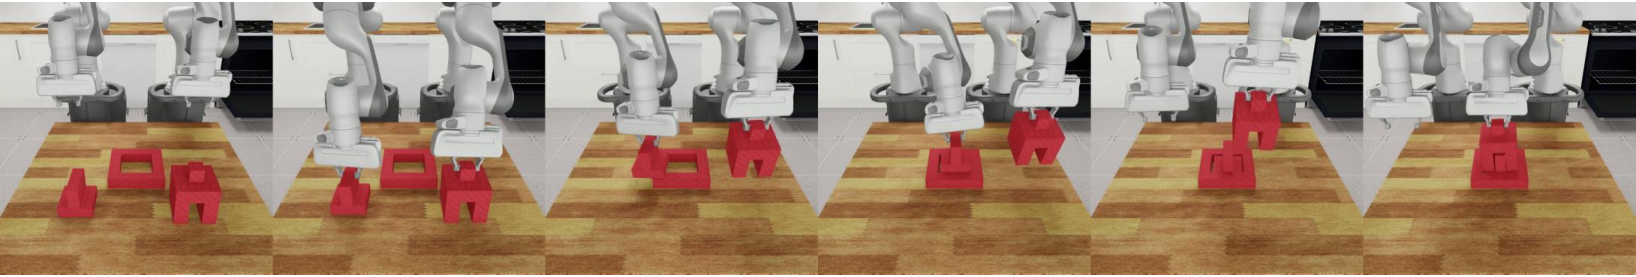
\includegraphics[width=0.94\textwidth]{figure/fig_assembly.pdf}\\[-2pt]
{\small\textbf{(a)} \textsc{PieceAssembly}}\par\vspace{2pt}
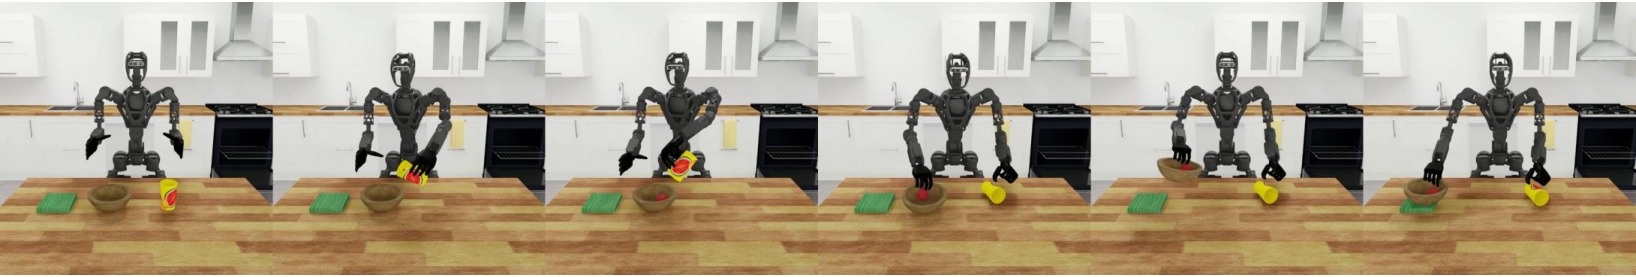
\includegraphics[width=0.94\textwidth]{figure/fig_pouring.pdf}\\[-2pt]
{\small\textbf{(b)} \textsc{Pouring}}\par\vspace{2pt}
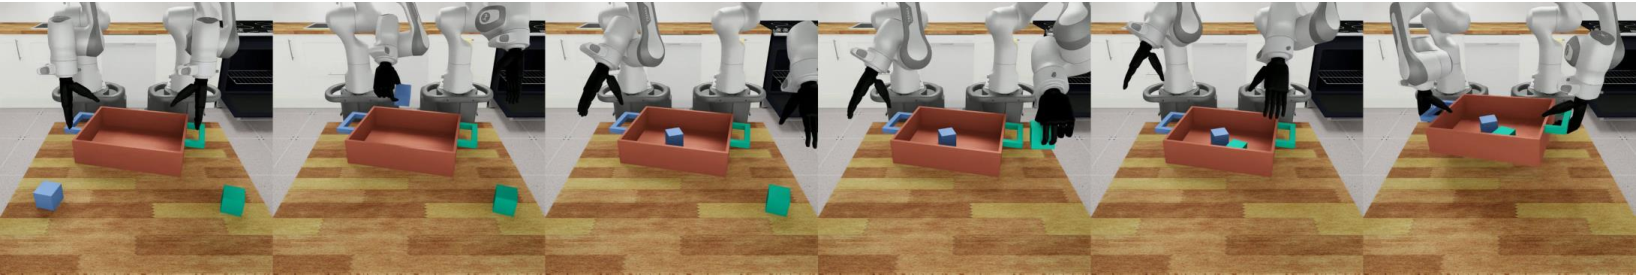
\includegraphics[width=0.94\textwidth]{figure/fig_lift_tray.pdf}\\[-2pt]
{\small\textbf{(c)} \textsc{LiftTray}}\par\vspace{2pt}
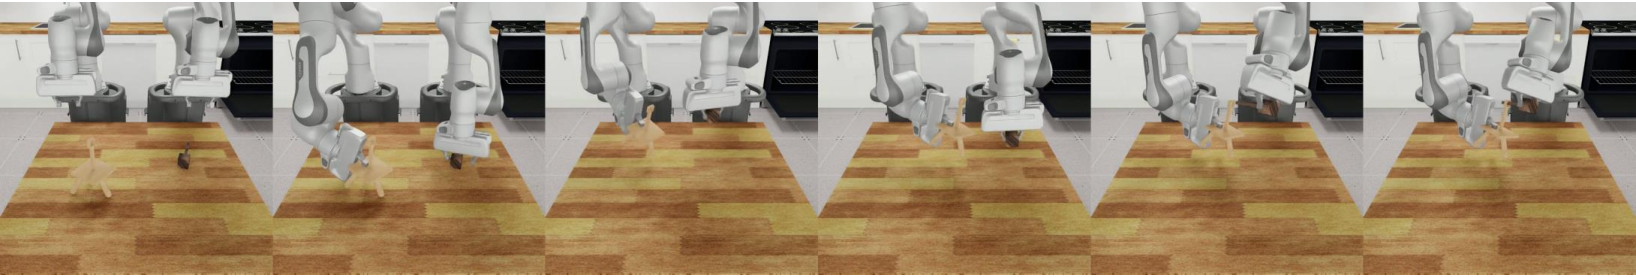
\includegraphics[width=0.94\textwidth]{figure/fig_threading.pdf}\\[-2pt]
{\small\textbf{(d)} \textsc{Threading}}\par\vspace{2pt}
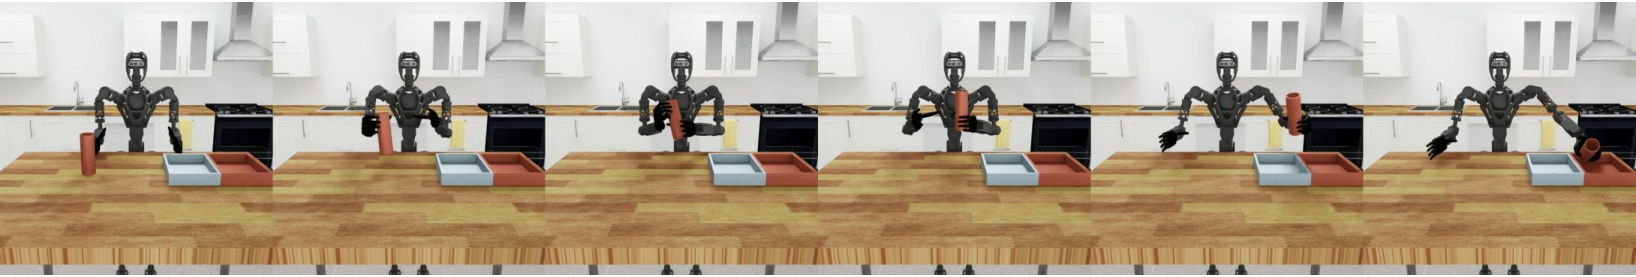
\includegraphics[width=0.94\textwidth]{figure/fig_can.pdf}\\[-2pt]
{\small\textbf{(e)} \textsc{CanSort}}\par
\caption{Representative execution sequences for the five simulated
DexMimicGen tasks. Each row proceeds from left to right. Panels (a)--(d) show
the four compositionally long-horizon tasks, while (e) shows the single-stage
control task.}
\label{fig:sim-task-processes}
\end{figure*}

\paragraph{LIBERO single-arm extension.}
We evaluate LIBERO-10 task ID~8 (instruction: \emph{put both moka pots on the
stove}) and LIBERO-90 task ID~57 (instruction: \emph{pick up the cream cheese
and put it in the tray}). Both tasks use a single arm, a $7$-D action space, and
visual-proprioceptive observations comprising $8$-D robot proprioception and two RGB
views (an agent view and the wrist view
\texttt{robot0\_eye\_in\_hand}). No object state or other privileged simulator
variable is provided to the policy. An episode terminates on the first task
success or is truncated at $520$ steps on LIBERO-10 and $400$ steps on
LIBERO-90.

\subsection{B.2\quad Base Policies and Frozen Features}

On the dual-arm tasks, the base policy is ACT~\cite{zhao2023learning}, fine-tuned
\emph{separately for each task} on its demonstrations and then frozen. On LIBERO, the
base is a served $\pi_0$ VLA~\cite{black2024pi0}, which is likewise frozen. In the
default and deployed configurations, the value modules read the base policy's
\emph{frozen} encoder feature $\psi_b$ together with proprioception, but no privileged
object pose. The residual actor and critic do not share this feature extractor; they
train their own multi-view encoder directly from the raw camera observations
(Section~A.4).

For ACT, $\psi_b$ is the mean-pooled encoder-token feature (width $512$). Concatenating
proprioception gives an input dimension of $530$ for
\textsc{PieceAssembly} and \textsc{Threading} ($512{+}18$), $548$ for
\textsc{Pouring} ($512{+}36$), and $550$ for \textsc{LiftTray} ($512{+}38$).
For $\pi_0$, $\psi_b$ is the last prefix token (width $2048$), extracted server-side
when the feature cache is built. Concatenating the standardized $8$-D LIBERO
proprioception gives a $2056$-D input.

The frozen base emits action chunks that are executed open-loop for $10$ steps between
replans. We also evaluated a $30$-step LIBERO setting as an execution-cadence
diagnostic; it is not part of the headline comparison. Ablation~D deliberately replaces
the default feature with a privileged $30$-D end-effector\,$+$\,object state
(\texttt{eef\_piece}) to provide an upper-bound reference. This ablation is the only
use of privileged object state; every deployed representation remains
visual-proprioceptive.

\subsection{B.3\quad Configuration and Hyperparameters}

The goal-conditioned value $V_{\mathrm{gc}}$ and navigator $\pi_h$ are
pretrained once per task from demonstrations using the frozen base-policy
features $\psi_b$. In all waypoint-enabled runs, including the dual-arm and
LIBERO runs, the two value heads and $\pi_h$ are then jointly fine-tuned during
residual RL while the bottleneck encoder $\phi$ remains frozen. These online
updates use Adam with a learning rate of $10^{-5}$ for both modules, a batch
size of $256$ split evenly between demonstrations and online data, and begin
after $2{,}000$ online transitions; one joint update is applied per residual
UTD block. The online navigator update aggregates the two value heads by their
minimum.

The separate single-state value that supplies $\Phi_V$ is trained independently from
demonstrations using only the current state, and remains frozen throughout residual
training. Table~\ref{tab:simvalue} reports the value and navigator settings, including
the architectural differences between the dual-arm and LIBERO instantiations.
Table~\ref{tab:simresrl} gives the residual-RL configuration; its venue-independent
core matches Table~\ref{tab:sharedhp}. Section~C.5 separately identifies the optimizer
settings reused in imagination and the collection settings that change. Together,
these values instantiate the general update in Section~A and the simulator version of
Algorithm~\ref{alg:shore}.

\begin{table}[t]
\centering\small\setlength{\tabcolsep}{4pt}
\begin{tabular}{@{}p{0.43\columnwidth}p{0.51\columnwidth}@{}}
\toprule
Setting & Value \\
\midrule
GC encoder/value MLPs (dual-arm)     & $3\times512$, LayerNorm$+$GELU \\
GC encoder/value MLPs (LIBERO)       & $2\times256$, LayerNorm$+$GELU \\
\quad bottleneck input               & $[g,s]$ dual-arm / $g$ LIBERO \\
\quad value heads / target           & $2$ / per-head HIQL bootstrap \\
Single-state $V(s)$ MLP              & $2\times256$, ReLU (separate net) \\
Waypoint bottleneck dim.\ $z$        & $10$ (bottleneck radius $\sqrt{10}$) \\
Deployment navigator mean             & raw dual-arm / radius-$\sqrt{10}$ renorm. on LIBERO only \\
Navigator $\pi_h$                    & $2\times256$, ReLU \\
\quad AWR inverse temp.\ $\beta$      & $1.0$ (weight clipped at $100$) \\
Waypoint horizon $k$                 & $15$ dual-arm / $25$ LIBERO \\
Expectile $\tau$                     & $0.7$ \\
Discount $\gamma$                    & $0.99$ \\
Target EMA                           & $0.005$ \\
Value goal mixture                   & current $0.2$/future $0.5$/random $0.3$ \\
\quad future-state offset            & geometric with parameter $1{-}\gamma$ \\
Offline navigator target             & clamp-to-goal; random-goal prob.\ $0.3$ \\
\quad advantage aggregation          & mean of $V_1,V_2$ \\
Goal-conditioned reward              & $0$ at the goal, $-1$ otherwise \\
Single-state $V(s)$ reward           & $1$ at final step, $0$ otherwise \\
Offline optimizer / lr               & Adam / $3{\times}10^{-4}$ \\
Offline steps / batch                & $50{,}000$ / $256$ \\
\bottomrule
\end{tabular}
\caption{Value and navigator configuration. The dual-arm
\texttt{hiqlv512} recipe uses $3\times512$ MLPs and \texttt{sg15} sets
$k=15$; the LIBERO instantiation uses $2\times256$ MLPs and $k=25$.
The single-state potential value is a separate state-only network.}
\label{tab:simvalue}
\end{table}

\begin{table}[t]
\centering\small\setlength{\tabcolsep}{4pt}
\begin{tabular}{@{}p{0.40\columnwidth}p{0.54\columnwidth}@{}}
\toprule
Setting & Value \\
\midrule
Regime                          & RLPD, TD3-style updates \\
Critic ensemble                 & $10$ Q-nets; target $=\min$ of $2$ random heads \\
Critic / actor MLP              & $2$ layers $\times$ $1024$, ReLU, LayerNorm \\
Residual actor output           & $\mu_\theta=s_a\tanh(f_\theta)$; final layer zero-init \\
Action scale $s_a$              & $0.05$ \\
Discount $\gamma$ / $n$-step    & $0.99$ / $3$ \\
Update-to-data (UTD)            & $4$ (actor updated every $4$th critic step) \\
Target Polyak $\tau$            & $0.005$ \\
Exploration / target noise      & $0.05$ (scaled coords), smoothing clip $0.3$ \\
actor\_lr / critic\_lr          & $1{\times}10^{-6}$ / $1{\times}10^{-4}$ (AdamW) \\
Batch / replay buffer           & $256$ / $2{\times}10^{5}$ \\
Offline demo fraction           & $0.5$ (RLPD demo mixing) \\
Demo-BC coefficient             & $0.1$ (MSE in scaled-action coords; no $1/s_a$, no clip) \\
Learning starts                 & $10^{4}$ \\
Total env.\ steps               & $5{\times}10^{5}$ \\
Potential $\Phi_V=c\,V(s)$      & $c=\frac{\max(K-1,\,1)}{\max(V_{\max}-V_{\min},\,10^{-6})}$ for $K$ stages; multiplier $1.0$ \\
Stage bonus (main)              & direct $+1$ per stage advance, stage-balanced replay \\
Gradient clip                   & $1.0$ \\
Eval                            & $50$ ep.\ (DexMimicGen) / $10$ (LIBERO) \\
\quad                          & $8$ envs, deterministic ($\sigma{=}0$) \\
\bottomrule
\end{tabular}
\caption{Residual off-policy RL configuration in simulation. The update combines
RLPD's $10$-head critic ensemble and $50/50$ demonstration mixing with TD3-style
target smoothing and delayed actor updates. The residual actor's final layer is
zero-initialized, so its deterministic output is exactly zero at step $0$; the
leftmost evaluation therefore measures the frozen base (Section~B.4).}
\label{tab:simresrl}
\end{table}

\subsection{B.4\quad Baselines}

We report a frozen-base reference, four external methods, and the component
ablations below. A cross-method comparison is \emph{matched} only if it shares the
base, offline data, budget, execution horizon, evaluation harness, and seed policy
of Section~B.6. \emph{BC base} is the frozen policy without RL; because the
deterministic residual is initially zero (Section~B.3), it is the leftmost evaluation
point of each run under the same task-specific protocol. \emph{Flat
residual}~\cite{resfit2025residual} removes the waypoint and shaping; we distinguish
the collapse-control setting BC$0$ from the demo-anchored BC$0.1$ setting.
\emph{DSRL}~\cite{wagenmaker2025dsrl} learns the correction in the same frozen
base's noise space. \emph{IBRL}~\cite{hu2023imitation} selects between base and
learned actions by a $Q$-argmax, providing a soft anchor. We instantiate this
selection rule on our RLPD/TD3 base and use the same evaluation harness as the
other dual-arm comparisons. All IBRL runs reach $500$k steps, with three
seeds per task. \emph{Full-policy
IQL}~\cite{kostrikov2022iql} instead fine-tunes the entire policy without a frozen
base, isolating the residual parameterization.

\subsection{B.5\quad Ablation Design}

Table~\ref{tab:simarms} gives the five-configuration structured component
study. Within a task, all configurations share the codebase, frozen features,
demonstrations, action scale, budget, and seed set. ``Waypoint'' includes
online joint fine-tuning of the two value heads and navigator. ``Stage'' is the
stage-derived training branch: it includes the direct bonus of Section~A.3 and,
where enabled, stage-balanced replay; it is not a potential-based reward.

\begin{table}[t]
\centering\small\setlength{\tabcolsep}{4pt}
\begin{tabular}{@{}lcccl@{}}
\toprule
Configuration & waypoint & BC & stage & Removed \\
\midrule
\textbf{Full (SHORE-RL)} & on  & $0.1$ & on  & --- \\
$-$ stage                & on  & $0.1$ & off & stage branch \\
$-$ waypoint             & off & $0.1$ & on  & waypoint \\
$-$ waypoint $-$ stage   & off & $0.1$ & off & waypoint $+$ stage \\
waypoint only             & on  & $0$   & off & BC $+$ stage branch \\
\bottomrule
\end{tabular}
\caption{Structured component ablation (Ablation~A). \textbf{Full} uses
waypoint$+$joint fine-tuning, demo-BC, and the stage-derived training branch;
each subsequent configuration removes the component(s) named in the last
column.}
\label{tab:simarms}
\end{table}

\paragraph{Shaping form.}
Ablation~B keeps waypoint$+$joint and BC$0.1$ fixed, and swaps only the direct stage
bonus for the self-derived potential $\Phi_V(s)$. It therefore tests removal of the
hand-designed detector without changing the rest of the method. The representation
comparison between privileged \texttt{eef\_piece} features and ACT or $\pi_0$ features
is orthogonal.

\paragraph{Coverage.}
The five component configurations cover \textsc{Pouring} and
\textsc{PieceAssembly}, with three seeds per configuration and a common
$4{\times}10^5$-step budget. The shaping-form pair covers
\textsc{PieceAssembly} and \textsc{Threading}, with three seeds per
configuration through $5{\times}10^5$ steps. \textsc{CanSort} is excluded
because its residual runs do not collapse and it has no stage decomposition.

\subsection{B.6\quad Evaluation Protocol}

All SHORE-RL and in-codebase ablation configurations use a common evaluator within each task.
We call a cross-method comparison \emph{matched} only when the base checkpoint,
offline demonstrations, execution horizon, success criterion, training budget, and
seed policy also agree. For the dual-arm tasks, evaluation uses an execution horizon
of $10$, eight parallel environments, and $50$ deterministic episodes per checkpoint;
LIBERO uses eight environments and $10$ episodes. For a success probability $p$, the
binomial standard error of a $50$-episode success-rate estimate is
$\sqrt{p(1-p)/50}\approx0.057$ at $p=0.8$; this within-checkpoint uncertainty is
distinct from the across-seed s.e.m.\ bands in the learning curves. The nominal online budget is
$5{\times}10^{5}$ environment steps for the main DexMimicGen comparison and
$4{\times}10^{5}$ environment steps for LIBERO; component Ablation~A uses the
matched $4{\times}10^{5}$-step budget stated above. Since the residual mean is zero
before training, the step-$0$ evaluation also provides the frozen-base reference.

Method-specific anchoring parameters---our action scale, DSRL's noise scale, and
IBRL's exploration scale---are calibrated only within the protocol used for the
corresponding comparison. The LIBERO DSRL overlay is the sole exception: it uses
DSRL's query-$20$ harness and is therefore indicative rather than strictly matched.
The IBRL comparison uses the matched dual-arm harness and the full $500$k-step
budget.

\paragraph{Reported metric.}
For each seed, the \emph{steady-state} success rate is the mean over its final $20\%$
of evaluation checkpoints. This window always contains at least one checkpoint. We then
report the mean and standard error of these seed-level values. Learning curves instead aggregate seeds at
each recorded checkpoint and show a $\pm1$ s.e.m.\ band when at least two seeds are
available. Diagnostic runs outside the matched main comparisons are shown only
over their observed ranges; their terminal windows are neither extrapolated nor
treated as budget-matched results.

\subsection{B.7\quad Results, Run Inventory, and Provenance}

The main paper reports the compact steady-state table and learning curves.
SHORE-RL and all four main baselines---the flat residual (ResFit), DSRL, IBRL,
and IQL---use three seeds per method on all four long-horizon tasks and reach
$500$k steps. The
\textsc{CanSort} diagnostic uses $2$--$3$ seeds per method, including three
completed IBRL seeds. Component
ablation~(A) covers \textsc{Pouring} and \textsc{PieceAssembly} with three
$400$k-step seeds per configuration. Shaping comparison~(B) uses three
$500$k-step seeds per configuration on
\textsc{PieceAssembly} and \textsc{Threading}. The LIBERO-10 Task~8 and
LIBERO-90 Task~57 studies use three $400$k-step seeds per method; the DSRL
comparison uses the separate harness described below.

\paragraph{Inclusion and provenance.}
The included dual-arm SHORE-RL, flat-residual, and ablation runs use the same
execution horizon ($10$) and eight-environment evaluator; legacy ablations evaluated
with one or four environments are excluded. Frozen-base references come only from
step-$0$ evaluations in the same harness and are never pooled across evaluator
settings or codebases.

Removing the waypoint also removes its online joint update and is therefore treated
as one bundled mechanism. A second, task-dependent caveat applies to the
structured component study: on \textsc{Pouring} and \textsc{PieceAssembly}, the
$-$stage configurations also disable stage-balanced replay and thus remove all stage-derived
training information. The shaping-form comparison is cleaner: all three seeds reach $500$k,
and only the direct stage bonus is replaced by the self-derived potential.

\paragraph{Coverage caveats.}
The main long-horizon comparison is complete and matched at three seeds and
$500$k steps for every method. IBRL's final-window performance is $0.00{\pm}0.00$ on
\textsc{Pouring}, \textsc{LiftTray}, and \textsc{Threading}, and
$0.10{\pm}0.05$ on \textsc{PieceAssembly}. The
smaller \textsc{CanSort} diagnostic uses the available $2$--$3$ seeds per
method, and the LIBERO DSRL overlay remains a separate-harness comparison, as
noted in Section~B.6.

\subsection{B.8\quad Limitations of the Simulation Venue}

\paragraph{Statistical coverage.}
The component ablation includes three matched $400$k-step seeds per
configuration on \textsc{Pouring} and \textsc{PieceAssembly}, and the
shaping-form comparison includes three full-budget seeds per configuration on
\textsc{PieceAssembly} and \textsc{Threading}. Their task coverage nevertheless
remains narrow: the evidence supports the reported component interactions and
the self-derived potential on these tested tasks, not universal equivalence or
task-independent effects. The smaller \textsc{CanSort} study is therefore
treated as a diagnostic rather than uniformly powered evidence.

\paragraph{Privileged task structure.}
The main simulation result uses a per-stage bonus computed from a task-specific
simulator predicate and thus applies only when a reliable stage decomposition is
available. The self-derived $V(s)$ potential removes this annotation requirement,
but its quality depends on the frozen value estimate and it need not recover a useful
progress signal on every task. This is why the real-robot venue uses the $V(s)$ form
throughout, while the simulation study reports both formulations.

\paragraph{Cross-method comparability and benchmark scope.}
The main dual-arm comparisons are matched within our evaluator. On LIBERO,
however, the DSRL overlay uses its own evaluation
harness, so absolute-success differences are indicative rather than strictly
controlled. The extension covers only LIBERO-10 Task~8 and LIBERO-90 Task~57
rather than the full LIBERO benchmark; claims about broader benchmark transfer
would require matched evaluation on additional tasks.

\section{C\quad Real-Robot Venue}

Everything in Section~B trains the residual against a cheap-to-step simulator. For
hardware evaluation we retain the residual parameterization and actor--critic objective of
Section~A, but instantiate its collector and replay sampler with a learned dynamics model
finetuned on our own robot data. This section documents that venue: the platform and its
interfaces (C.1), the three tasks and their success
criteria (C.2), the demonstration and rollout data (C.3), the dynamics model (C.4),
the imagination loop the residual is trained in (C.5), the protocol used to evaluate
the resulting residual on the physical robot (C.6), and the limitations specific to
this venue (C.8).

\subsection{C.1\quad Real-Robot Platform and Control}

\paragraph{Robot.}
The real-robot venue uses a full-body robot; control is over its two
$7$-DoF arms, each terminated by a parallel gripper. Commands are joint-space targets,
so the action space is $16$-dimensional, $(7\ \text{joints} + 1\ \text{gripper}) \times 2$.
The robot controller consumes one joint-space command per step at $30$\,Hz (matching
the camera rate), and commands are absolute joint-position targets rather than deltas.

\paragraph{Perception.}
Perception is image-only: three RGB cameras stream $848{\times}480$ video at
$30$\,Hz, consisting of one head-mounted view (\texttt{top\_head}) and two wrist-mounted views
(\texttt{hand\_left}, \texttt{hand\_right}). The same three views are consumed by
every component that needs to see the scene: the base policies, the frozen
encoder $\psi_b$ that supplies the value's state representation, and the dynamics
model. No component receives a signal the deployed robot does not have, because there is
no motion capture, no object pose, and no privileged state anywhere in this
venue.

\paragraph{Base policy and action chunking.}
Each task's base policy is a served $\pi_{0.5}$-style
VLA~\cite{sima2026kai0,black2025pi05} that
emits $50$-step
action chunks, executed open-loop within each chunk. Internally the VLA's action
vector is zero-padded to its native width of $32$ dimensions, of which the
leading $16$ are the platform's commands; the padding is stripped before
execution and before any residual is added.

\paragraph{What runs at deployment.}
At deployment the robot runs the task's frozen base policy, the navigator on
the frozen base features, and the residual actor on its separate trained
multi-view image encoder together with proprioception, the base action, and the
waypoint. The dynamics model is a training-time device only and is never
executed at inference time, so the deployed system carries no video dynamics
model; its additional computation is the residual encoder and actor plus the
navigator.

\begin{figure*}[tp]
\centering
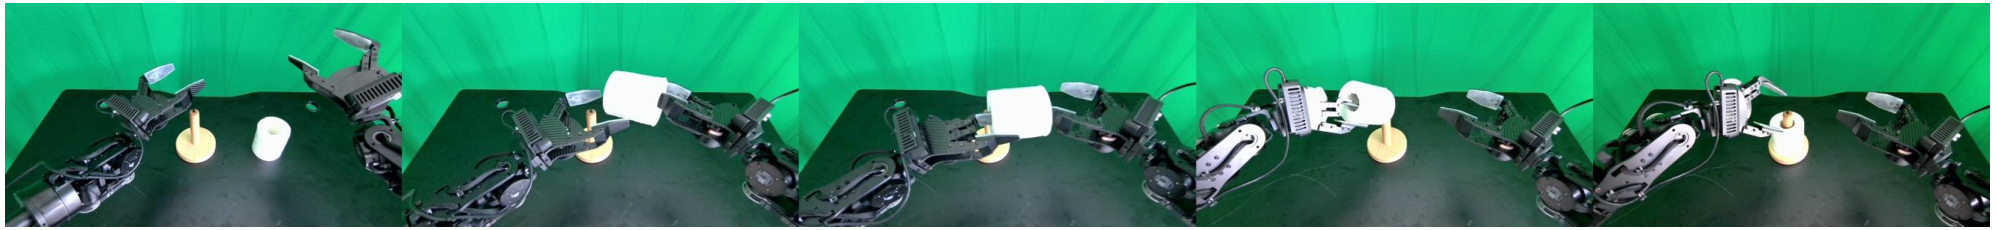
\includegraphics[width=0.96\textwidth]{figure/fig_roll.pdf}\\[-2pt]
{\small\textbf{(a)} \textsc{pick\_paper\_roll}}\par\vspace{3pt}
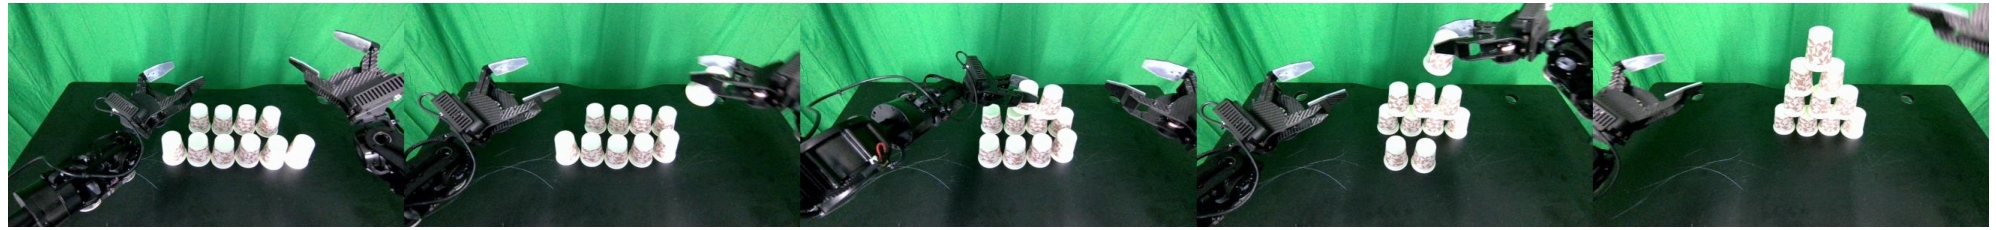
\includegraphics[width=0.96\textwidth]{figure/fig_cup.pdf}\\[-2pt]
{\small\textbf{(b)} \textsc{pick\_cup}}\par\vspace{3pt}
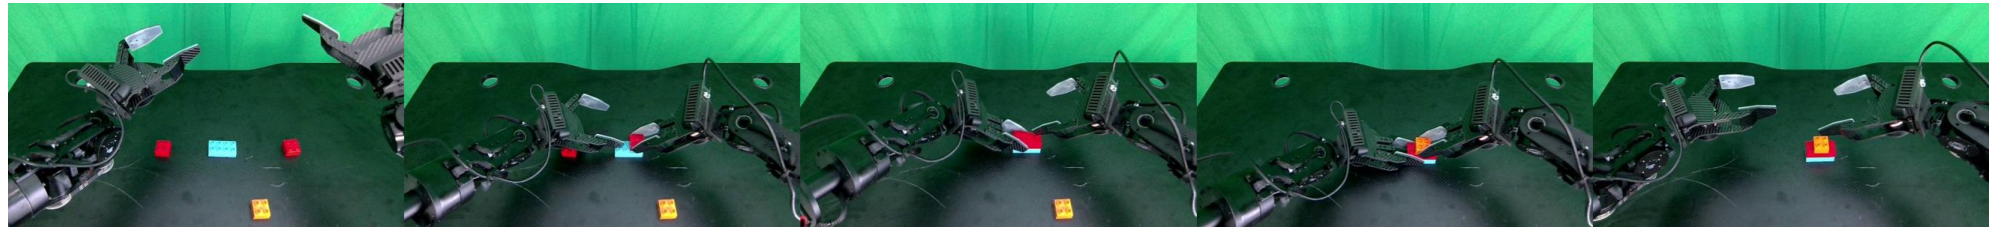
\includegraphics[width=0.96\textwidth]{figure/fig_block.pdf}\\[-2pt]
{\small\textbf{(c)} \textsc{build\_block}}\par
\caption{Representative execution sequences for the three real-robot tasks,
shown from left to right: (a) placing a paper roll on its holder, (b) manipulating
and arranging the cups, and (c) assembling the colored blocks.}
\label{fig:real-task-processes}
\end{figure*}

\subsection{C.2\quad Tasks and Success Criteria}

We evaluate on three tabletop bimanual tasks. The robot controller and cameras
operate at $30$\,Hz during physical evaluation. The dynamics-model training data
uses $30$\,Hz for \textsc{build\_block} and \textsc{pick\_cup}, while the
\textsc{pick\_paper\_roll} domain is made internally uniform at $20$\,Hz by
resampling its frozen-base rollouts (Section~C.4.2). Episodes end when the task
is completed or its task-specific timeout is reached.
\todo{report the physical-evaluation timeout and resulting trial-duration range
for each task.}
For each task we quote the language instruction verbatim as it appears in the
dataset, because that same string is the caption conditioning the dynamics model
(Section~C.4), and because a mismatch between the two would silently change what
the model is conditioned on. Representative physical-robot executions are shown
in Figure~\ref{fig:real-task-processes}.

\paragraph{\textsc{pick\_paper\_roll}} The instruction is \texttt{put the paper roll on
the holder}. The robot grasps a paper roll from the tabletop and places it onto
an upright holder. A key challenge is that the roll is a rolling object: a grasp
that is not centered displaces it rather than securing it, and the resulting
error compounds into the placement. The representative successful sequence in
Figure~\ref{fig:real-task-processes} starts with the roll upright and uses one
gripper to transport it directly to the holder; no inter-arm handover occurs.
\emph{Success}: the holder's vertical peg passes through the roll's central
opening, the roll rests on the holder base, and the gripper has released and
withdrawn.

\paragraph{\textsc{pick\_cup}} The instruction is \texttt{pick cup}. This is the
Cup Stacking task in the main paper. Ten upright paper cups start distributed
on the tabletop; the robot rearranges them into a four-level $4$--$3$--$2$--$1$
stack, so reorienting a fallen or sideways cup is not part of the demonstrated
task. \emph{Success}: all ten cups form the required four-level structure and
remain stable after the grippers release and withdraw.

\paragraph{\textsc{build\_block}} The instruction is \texttt{build block}. This is an
assembly-style task. The representative sequence starts from four loose pieces
(two red, one cyan, and one yellow) and builds a three-piece vertical target:
cyan base, red middle, and yellow top, leaving the second red piece unused as a
distractor. \emph{Success}: the three target pieces form this assembly and it
remains intact after the grippers release and withdraw. \todo{confirm whether
this color order is fixed across the entire evaluation set and whether each arm
is assigned particular pieces.}

\paragraph{Randomization.}
Object placements vary across episodes. Physical evaluation uses a fixed
initial-state set shared across the compared conditions. \todo{confirm the
training randomization protocol---which objects are randomized, over what
region, and whether the robot's initial pose is randomized---and report how the
fixed evaluation set was constructed and whether it is held out from the
training-placement distribution.}

\paragraph{Why binary success.}
We score each trial with a single binary criterion rather than a per-stage
rubric. This keeps the real-robot metric identical in kind to the simulated one
and avoids introducing stage labels into a venue whose entire point is that it
runs without them: the shaping potential here is the self-derived single-state
value, precisely because no stage detector is available on hardware.

\subsection{C.3\quad Demonstration and Rollout Data}

Two kinds of data are collected on the physical robot, and they enter the
pipeline at different points.

\paragraph{Expert demonstrations.}
For each task we collect about $1{,}000$ successful human-teleoperation
episodes, stored in LeRobot format with per-frame images, joint states, and
actions. These train the base policies: we finetune the $\pi_{0.5}$ VLA
\emph{separately per task}, giving one base policy per task, each frozen from
that point on.

\paragraph{Base-policy rollouts.}
We then deploy each frozen base on the physical robot and record its rollouts.
These are mixed-outcome by construction, in that they contain exactly the residual
failures that the base policy has not overcome, and they are used only for the
dynamics model, never for base-policy training. This is deliberate: the model
must be able to render the failure modes the residual is being trained to avoid,
and a model finetuned on success-only data cannot, because it has never seen one.

\begin{table}[t]
\centering\small\setlength{\tabcolsep}{4pt}
\begin{tabular}{@{}lrrr@{}}
\toprule
Task & successful teleoperation & base rollout & Hz \\
\midrule
\textsc{build\_block}      & $\sim1{,}000$ & $50$ & $30$ \\
\textsc{pick\_cup}         & $\sim1{,}000$ & $51$ & $30$ \\
\textsc{pick\_paper\_roll} & $\sim1{,}000$ & $53$ & $20$ \\
\bottomrule
\end{tabular}
\caption{Real-robot data scale, per task. Each task is one dynamics-model
domain (\texttt{block}, \texttt{cup}, and \texttt{paper}, respectively;
Section~C.4.2). Successful human teleoperation trains the task-specific base;
recorded frozen-base rollouts enter only dynamics-model finetuning. The main
paper's approximately $1{,}000$ successful demonstrations per task is the
authoritative collection count. \todo{reconcile the filtered local pipeline
inventory with the full collection and then report exact per-task demonstration
counts and merged frame totals.}}
\label{tab:realdata}
\end{table}

\subsection{C.4\quad Dynamics Model}

\subsubsection{C.4.1\quad Architecture and Action Conditioning}

The dynamics model $D$ predicts the next $H$ multi-view frames from an
observation history and an action chunk. We instantiate it as an
action-conditioned multi-view video-diffusion model and finetune it from a
publicly released checkpoint pretrained on large-scale robot-manipulation
video~\cite{yang2026rise}, following that work's training recipe.

The backbone is an LTX-Video~\cite{hacohen2025ltxvideo} stack, comprising a T5~\cite{raffel2020t5} text encoder, a causal video VAE, and a
$28$-layer diffusion transformer ($32$ attention heads of dimension $64$,
cross-attention width $2{,}048$, $128$ latent channels), and it is trained with a flow-matching
objective~\cite{lipman2023flowmatching} under logit-normal timestep weighting. Each training sample is
$3$ views $\times$ $[\,4\ \text{history} + 25\ \text{predicted}\,]$ frames at
$256{\times}192$, downsampled from the native $848{\times}480$, paired with the
$50$-step action chunk that spans the predicted window.

During dynamics-model finetuning, actions are normalized using the statistics
specified by the training configuration. The retained \textsc{build\_block}
imagination launcher, however, does not provide an
\texttt{action\_norm\_json}. Its bridge therefore uses fixed per-dimension
bounds of $[-1,1]$, samples action indices $0,2,\ldots,48$ from each
$50\times16$ chunk, zero-pads the $16$ channels to $30$, and sends a bf16 tensor
of shape $1\times25\times30$. The stored step-$18{,}000$ checkpoint contains
the action-conditioning path, but its exact initialization provenance is not
retained locally. The action embedding is added to the caption embeddings that
drive cross-attention, a comparatively weak form of conditioning; action
controllability must therefore be tested rather than assumed
(Section~C.4.4).

\subsubsection{C.4.2\quad Mixed-Quality Training Data and Shortcut Controls}

The available finetuning configuration specifies a \emph{single} dynamics model
and a joint full-parameter update over the pooled data of all three tasks. The
asymmetry with the base policies, which are one per task against a single
shared dynamics model, is deliberate: predicting how a scene responds to an
action chunk is largely task-independent and benefits from pooling, whereas the
policies do not.

The data is organized as three domains, one per task, each containing that task's
expert demonstrations \emph{and} that task's base-policy rollouts merged into a
single dataset (Table~\ref{tab:realdata}). Because the model has no notion of
success or failure, its objective being pure video prediction, mixing the two is
what teaches it to render failure at all.

That mixing, however, creates an opportunity for the model to learn a shortcut
instead of dynamics, and we control for two such shortcuts explicitly.

\paragraph{(i) Frame rate, within a domain.}
The \textsc{pick\_paper\_roll} expert data is recorded at $20$\,Hz while its
failure rollouts were recorded at $30$\,Hz. The loader samples windows by
\emph{frame count}, not by wall-clock duration, and the model is never told the
frame rate, since its temporal position encoding is the bare frame index. A
within-domain frame-rate difference would therefore make inter-frame motion
magnitude collinear with success versus failure, letting the model infer the
outcome from apparent speed rather than from the action-conditioned dynamics,
which is exactly the capability the negative probe of Section~C.4.4 is meant to
test. We resample the failure rollouts to $20$\,Hz so that the domain is
internally uniform. The remaining \emph{across}-domain difference
($20$\,Hz for \texttt{paper} versus $30$\,Hz for \texttt{block} and
\texttt{cup}) is left as is: it is collinear with the task, not with the
outcome, and task identity is already supplied to the model through the caption.

\paragraph{(ii) Caption, within a domain.}
For the same reason, all episodes within a domain carry one identical caption, so
text cannot serve as a success/failure indicator. This required unifying the
\texttt{block} domain, whose expert and rollout splits had been captioned
differently, onto the single string \texttt{build block}.

\paragraph{Scope of the retained launcher.}
The retained block imagination launcher does not finetune the dynamics model.
It connects the learner to a model that must already be served at port 9000.
The retained service log shows a load from \texttt{block\_infer.yaml} and the
step-$18{,}000$ diffusion checkpoint. However, the websocket metadata contains
only a generic model name and the camera list, and the run's
\texttt{bridge\_run\_config.json} does not record the server configuration or
checkpoint digest. The launch record therefore establishes the inference path
below, but not the pooled three-domain training provenance or an immutable
run-level binding to that checkpoint. Those require a separate
dynamics-training record.

\subsubsection{C.4.3\quad Finetuning Configuration}

The available finetuning configuration specifies a single joint,
full-parameter update over the pooled data of all three domains.
Table~\ref{tab:wmhp} lists its settings.

\begin{table}[t]
\centering\small\setlength{\tabcolsep}{4pt}
\begin{tabular}{@{}ll@{}}
\toprule
Setting & Value \\
\midrule
Initialization      & released pretrained checkpoint \\
Objective           & flow matching (logit-normal weighting) \\
Views               & $3$ (head, left wrist, right wrist) \\
Frames per sample   & $4$ history $+$ $25$ predicted \\
Resolution          & $256{\times}192$ \\
Action chunk        & $50$ steps, per-domain normalized \\
Optimizer           & AdamW, $\beta=(0.9, 0.95)$ \\
Learning rate       & $1{\times}10^{-4}$, constant \\
Warmup steps        & $2{,}000$ \\
LR scaling by batch & none \\
Precision           & bf16, gradient checkpointing \\
Sharding            & DeepSpeed ZeRO-2 \\
Batch size          & $4$ per GPU ($48$\,GB) / $8$ per GPU ($96$\,GB) \\
Training steps      & $18{,}000$ (checkpoint used downstream) \\
Caption dropout     & $0.06$ \\
First-frame noise   & $0.2$ \\
Validation          & every $1{,}000$ steps (per-domain videos) \\
Checkpoint          & every $2{,}000$ steps \\
\bottomrule
\end{tabular}
\caption{Available finetuning configuration associated with the
step-$18{,}000$ artifact loaded by the retained \textsc{build\_block} service.
The imagination launcher performs inference only and does not itself record or
verify the served checkpoint identity or pooled-data provenance.
\todo{report the dynamics-model finetuning hardware and wall-clock time.}}
\label{tab:wmhp}
\end{table}

\begin{table}[t]
\centering\small\setlength{\tabcolsep}{4pt}
\begin{tabular}{@{}ll@{}}
\toprule
Retained block inference field & Value \\
\midrule
Service configuration & \texttt{block\_infer.yaml} \\
Loaded model & diffusion checkpoint, step $18{,}000$ \\
Checkpoint SHA-256 & \texttt{9b07acec$\ldots$69f8a} \\
Transformer parameters & $1{,}990{,}672{,}572$ \\
Prompt & \texttt{build block} \\
History tensor & $3\times3\times4\times192\times256$ \\
Action-token tensor & $1\times25\times30$ (bf16) \\
Inference steps & $10$ \\
Returned prediction & $3\times3\times25\times192\times256$ \\
\bottomrule
\end{tabular}
\caption{Code-backed inference contract for the retained block launch with
training GPU~7 and seed~0. The service returns $29$
frames per view including the four conditioning frames; the bridge removes
those frames and retains the $25$ predicted frames reported here. The digest is
the locally verified SHA-256 prefix and suffix of the loaded model artifact.}
\label{tab:block-wm-runtime}
\end{table}

\subsubsection{C.4.4\quad Qualitative Inspection and Available Monitoring}

The dynamics model is the environment in this venue, so failures of the dynamics
model become failure modes of the residual. A complete validation protocol
should therefore cover three complementary axes before any policy training.
Figure~\ref{fig:supp-wmval} reports the currently available qualitative evidence
for the first axis on one successful recorded episode from each task. The
retained launcher does \emph{not} implement a held-out dynamics-model
validation: its scheduled evaluator instead rolls the current residual policy
inside the same imagination environment and start-state pool used for
training. The held-out aggregate evaluation and the remaining two axes are
therefore left explicit below.

\paragraph{(i) Imagined-rollout quality.}
Given a real observation history and the ground-truth action chunk that follows
it, the imagined $H$-step future is compared against the recorded future.
For each task, Figure~\ref{fig:supp-wmval} shows representative, temporally
corresponding head-camera observations from the recorded and predicted futures.
The displayed moments are selected separately for each task, rather than using
a shared fixed-step schedule. Agreement in object layout, manipulator motion,
and task progression provides a direct qualitative check of rollout quality.
The dynamics model predicts all three camera views, but only the head view is
shown here for readability.

\paragraph{(ii) Action controllability, including a negative probe.}
The same observation history under different action chunks must yield
\emph{diverging} futures; a model that ignores its action input is a video prior,
not a dynamics model, and would make the residual gradient meaningless. The
sharper form of this test is the negative probe: we feed deliberately perturbed
actions, such as translating the grasp segment by a few centimeters or closing the gripper
early. The imagined video must show the corresponding failure rather than a hallucinated
success; examples include a missed grasp or a slip. Passing this probe is the entire reason the
mixed-quality data of Section~C.4.2 exists; failing it means the failure fraction
or the training budget is insufficient.

\paragraph{(iii) Potential-trajectory consistency.}
Finally we check the quantity the residual actually optimizes, rather than
pixels: $V(\psi(\hat{o}_{t+k}))$ must track $V(\psi(o_{t+k}))$ over $k$. A model
can be visually plausible and still be useless here if the re-encoded imagined
frames land where the potential misreads them, so this is the axis that most
directly predicts whether imagination training transfers.

\todo{P0: report the held-out split size and a quantitative rollout metric for
(i), then run and report the action-perturbation probe in (ii) and the
potential-trajectory comparison in (iii).}

\paragraph{What the retained launch actually records.}
At the first collected chunk (step $50$) and then every $50{,}000$ reported
control steps through step $500{,}000$, the evaluator saves a checkpoint and
generates ten two-segment imagined rollouts. Each rollout contains $50$
predicted frames. The resulting JSONL artifact contains $110$ trajectories and
$5{,}500$ frame scores from a \emph{separate} frozen value model. Table~
\ref{tab:block-proxy} reports the final-frame proxy. It is a continuous
training-time diagnostic, not a success classifier, a real-robot success rate,
or a held-out world-model metric. The evaluator deliberately returns
\texttt{eval/success\_rate=0.0} only as a checkpointing placeholder; that field
must not be read as an observed $0\%$ success rate.

\begin{table}[t]
\centering\small\setlength{\tabcolsep}{6pt}
\begin{tabular}{@{}rrr@{}}
\toprule
Reported step & Mean final proxy & Population SD \\
\midrule
$50$      & $0.617$ & $0.194$ \\
$50$k     & $0.560$ & $0.218$ \\
$100$k    & $0.317$ & $0.571$ \\
$150$k    & $0.473$ & $0.348$ \\
$200$k    & $0.396$ & $0.413$ \\
$250$k    & $0.262$ & $0.370$ \\
$300$k    & $0.471$ & $0.288$ \\
$350$k    & $0.329$ & $0.474$ \\
$400$k    & $0.463$ & $0.473$ \\
$450$k    & $0.442$ & $0.303$ \\
$500$k    & $0.496$ & $0.354$ \\
\bottomrule
\end{tabular}
\caption{Training-time imagined value-proxy record for the retained
\textsc{build\_block}, seed-$0$ run ($10$ rollouts per checkpoint). The
evaluator samples from the training start-state pool, records no episode/frame
identifier or real future, and applies no calibrated success threshold.
Accordingly, these values are monitoring diagnostics only.}
\label{tab:block-proxy}
\end{table}

\begin{figure*}[tp]
\centering
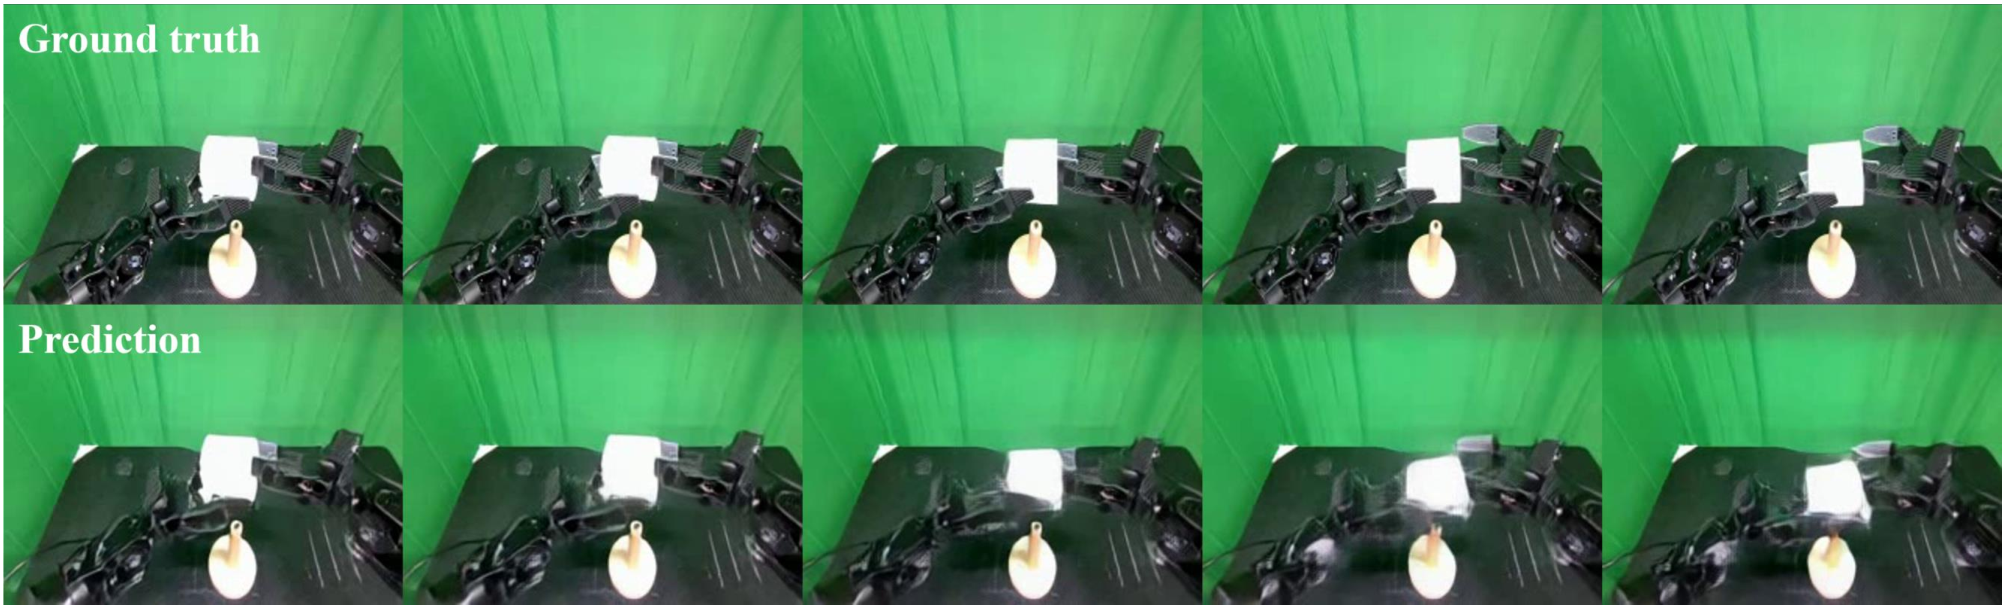
\includegraphics[width=0.96\textwidth]{figure/fig_world_model_paper.pdf}\\[-2pt]
{\small\textbf{(a)} \textsc{pick\_paper\_roll}}\par\vspace{3pt}
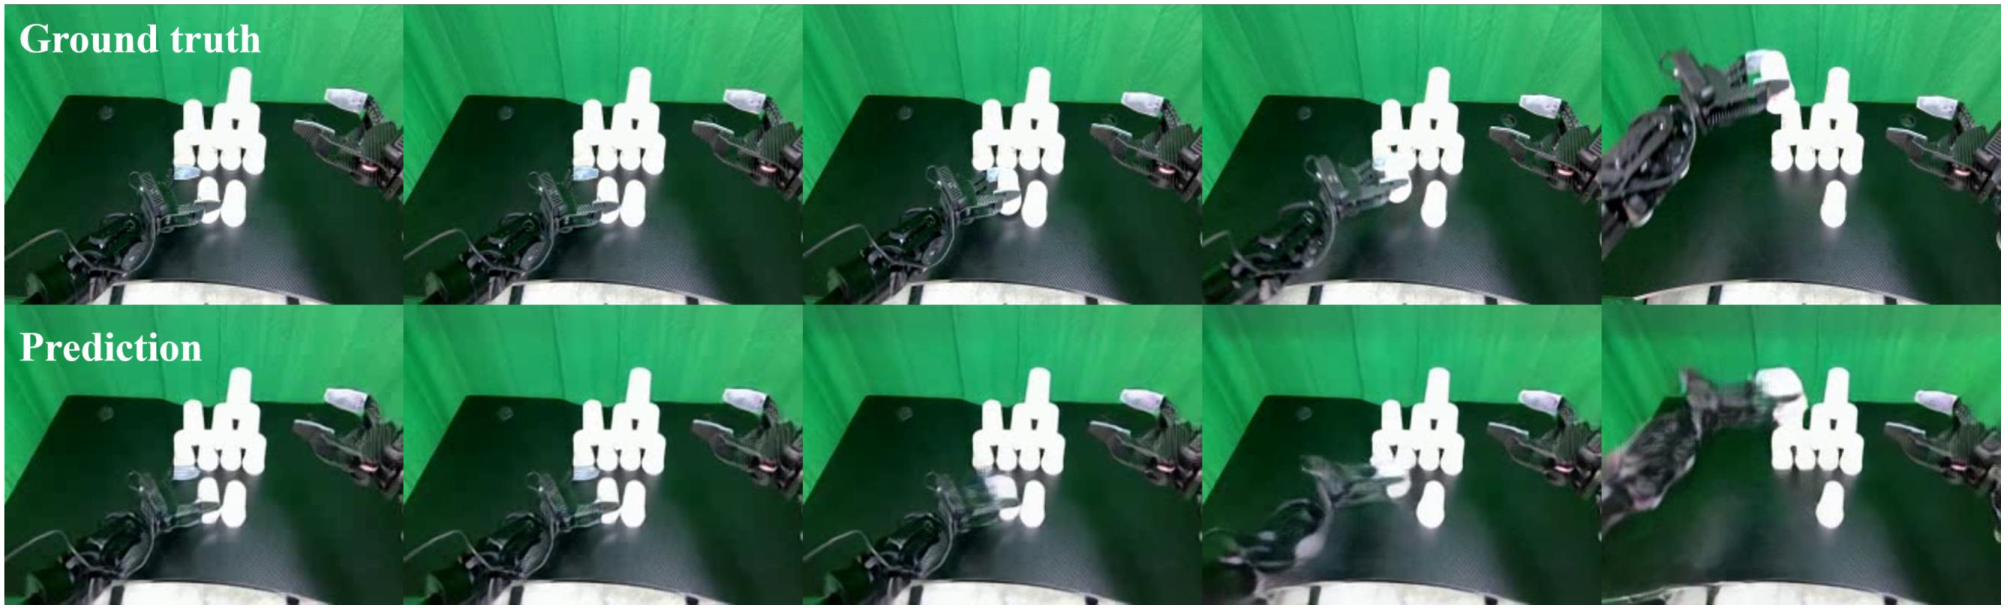
\includegraphics[width=0.96\textwidth]{figure/fig_world_model_cup.pdf}\\[-2pt]
{\small\textbf{(b)} \textsc{pick\_cup}}\par\vspace{3pt}
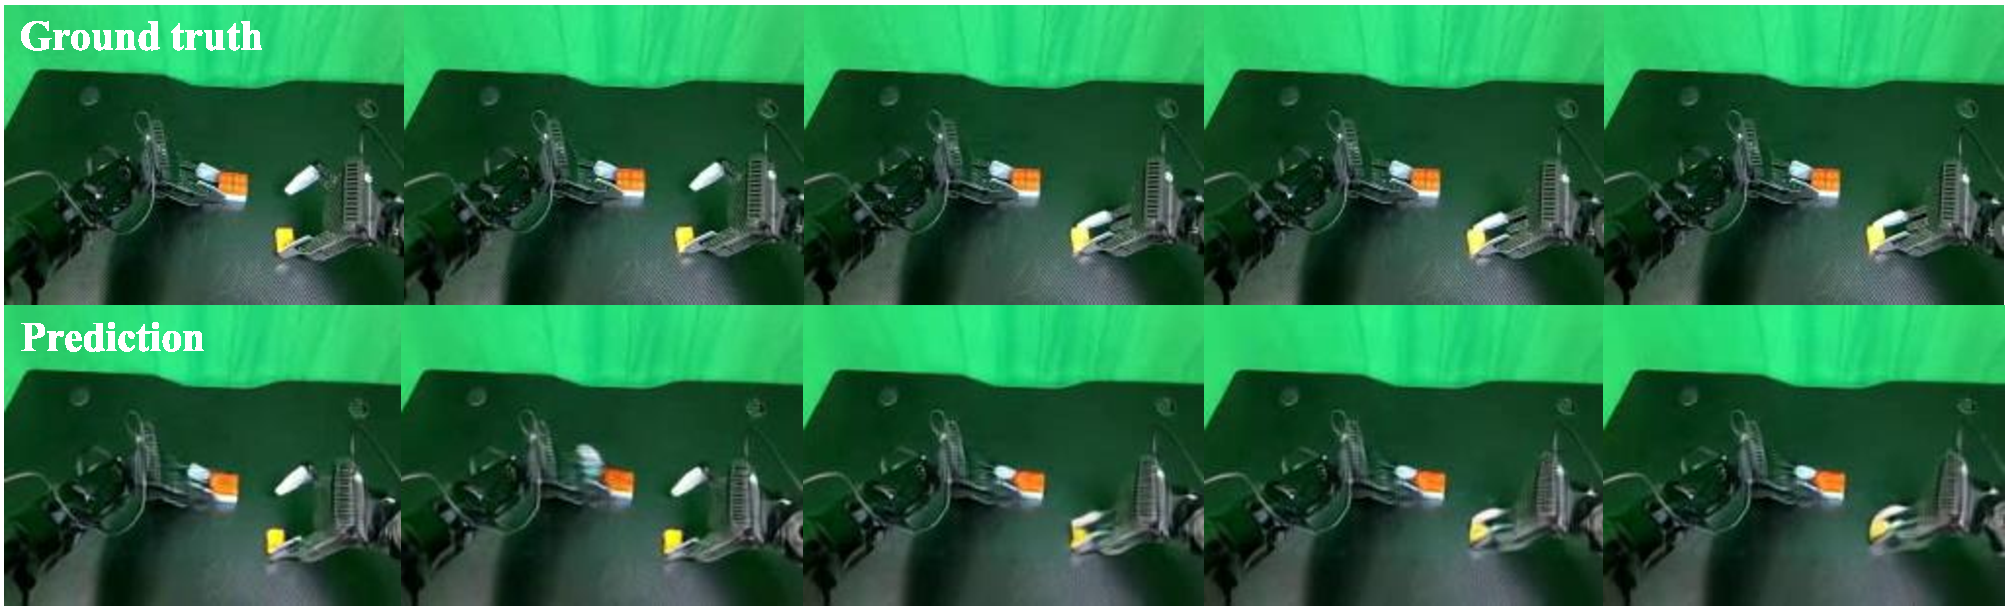
\includegraphics[width=0.96\textwidth]{figure/fig_world_model_block_outlined.pdf}\\[-2pt]
{\small\textbf{(c)} \textsc{build\_block}}\par
\caption{\textbf{Qualitative action-conditioned rollout comparison.}
One successful recorded episode is shown for each real-robot task:
(a)~\textsc{pick\_paper\_roll}, (b)~\textsc{pick\_cup}, and
(c)~\textsc{build\_block}. Each panel compares representative head-camera
observations from the recorded future (top) and the dynamics-model prediction
(bottom), conditioned on the same observation history and recorded action
sequence. The displayed moments are selected separately for each task and do
not follow a shared fixed-step schedule. These examples provide qualitative
evidence for rollout correspondence only. They are not generated by the
residual-training launcher and do not replace the pending held-out quantitative
metric, action-perturbation probe, or potential-trajectory comparison.}
\label{fig:supp-wmval}
\end{figure*}

\subsection{C.5\quad Residual RL in Imagination}

\paragraph{Exact scope of the retained block command.}
The following implementation record is for
the block launcher with training GPU~7 and seed~0. Despite the output-directory
label containing ``shore,'' its recorded trainer configuration uses the raw
actor and disables subgoal conditioning, stage conditioning, relabeling,
online value finetuning, and online high-actor finetuning. Thus this exact
artifact is a flat, non-waypoint-conditioned residual run: it contains no
$z_t$, no online $V_{\mathrm{gc}}$ update, and no navigator $\pi_h$ update. A
waypoint-conditioned SHORE-RL real-robot result cannot be attributed to this
command without a separate matching launch configuration and artifact.

\paragraph{Synchronous segment generation and replay.}
A video-diffusion model is too slow to run at the robot's control frequency,
so the implementation exposes it as a chunk-level rather than control-step
environment. The frozen base and flat residual produce a $50\times16$ action
chunk. After the outer wrapper accumulates all $50$ commands, $D$ consumes the
subsampled action tokens together with four history frames and predicts $25$
future frames for each of the three camera views. At the block dataset rate of
$30$\,Hz, one action chunk spans $1.667$\,s and the predicted frames are at
$15$\,Hz. The final predicted frame is re-encoded by the frozen base, scored
once, and stored immediately as one transition in the online imagination
replay. Generation and TD3~\cite{fujimoto2018addressing} updating therefore
alternate synchronously; there is no periodic $K$-update refresh or separately
generated batch of $M$ rollouts.

Each seed drawn from the recorded robot data is advanced for at most two
generated segments. At the second-segment boundary, the collector preserves the
generated endpoint as the replay bootstrap observation, marks the boundary as an
artificial truncation, and resets from a new recorded seed. Seeds are sampled
uniformly over the pooled episode list containing $295$ successful
demonstrations and $50$ frozen-base failure rollouts, followed by a uniform
valid four-frame window within the selected episode. The recorded failure
transitions themselves are not inserted into the training batch. This bounded
recursion gives each imagined rollout $100$ actions and $50$ predicted frames
($3.333$\,s at $30$\,Hz) before it is re-anchored to real data
~\cite{janner2019mbpo}. The sampler uses an unseeded
\texttt{numpy.random.default\_rng()} and does not record the sampled
episode/frame identifiers, so the command's seed $0$ does not make the exact
start-state sequence replayable.

The online replay has capacity $200{,}000$ chunk transitions. A separate offline
replay is built from the retained $295$ successful \textsc{build\_block}
demonstrations. It contains $6{,}989$ non-overlapping $50$-step transitions
plus a final aligned chunk where needed; no episode was skipped as too short.
\todo{reconcile this filtered replay artifact with the full demonstration
collection summarized in Table~\ref{tab:realdata}.}
Every update samples $128$ imagined and $128$ demonstration
transitions, giving batch size $256$ and an offline fraction of $0.5$. Training
starts after $10{,}000$ reported control steps, equal to $200$ generated chunk
transitions, and first performs $10{,}000$ critic-only warmup updates. Thereafter
the update-to-data ratio is $4$, with a one-step target, $\gamma=0.995$, residual
scale $s_a=0.2$, and demonstration-BC coefficient $0.1$. The reported
$500{,}000$-control-step checkpoint corresponds to $10{,}000$ generated chunk
transitions. The launcher assigns four single-GPU processes: the dynamics-model
service on GPU~0, frozen-base service on GPU~1, monitoring-only advantage proxy
on GPU~6, and seed-$0$ learner on GPU~7. The retained online W\&B run
\texttt{eegyfzmz} (code commit
\texttt{b22fcbda$\ldots$b9a4}) records $18{,}798$\,s
($5.22$\,h) from W\&B initialization through step $500{,}000$; offline cache
construction occurred before that timer. Eleven persistent checkpoints were
saved at steps $50$, $50$k, $100$k, \ldots, $500$k, in addition to a rolling
latest checkpoint. The final retained checkpoint is step $500{,}000$.
\todo{report matching provenance and runtime for the other task runs.}
This loop implements synchronous chunk-level residual TD3 with a two-segment
imagination collector and a 50/50 demonstration--imagination replay mixture.

\paragraph{No task reward; self-derived endpoint potential only.}
The hand-designed per-stage bonus used in the main simulated results
(Section~B.3) reads simulator predicates that do not exist here. In the bridge,
the additive task-reward term is identically zero,
$r_t^{\mathrm{imag}}\equiv0$, and each completed imagined chunk receives
\[
\tilde r_t^{\mathrm{imag}}
=0+\gamma\Phi_V(\widehat e_{t+1})-\Phi_V(e_t),
\]
where $\gamma=0.995$ and $\Phi_V$ is a frozen ValueMLP evaluated on the
concatenation of mean-pooled frozen-base prefix features and proprioception.
The potential checkpoint has SHA-256
\texttt{1eb54786$\ldots$40411b}.
There is no imagined success classifier and no task-success terminal:
\texttt{terminated} is always false, while the second-segment boundary sets
\texttt{truncated=true}. The successful-demonstration replay uses the same
potential-only endpoint reward; only its final recorded chunk has
\texttt{done=true} and masks the critic bootstrap. An artificial imagination
boundary instead stores \texttt{done=false} and bootstraps from its preserved
generated endpoint. The trainer's \texttt{reward\_shaping=none} prevents a
second shaping pass; the logged \texttt{potential\_source=stage} option is
therefore inactive and does not indicate use of a stage detector. No physical
environment transition is executed during residual training.

\paragraph{What is frozen and what is trained.}
For this command, the task-specific base policy and its feature encoder
$\psi_b$, the dynamics model $D$, the single-state value supplying $\Phi_V$,
and the separate advantage-proxy monitor are frozen. Only the flat residual
actor and critic are trained. The waypoint bottleneck, goal-conditioned value,
and navigator are not instantiated in this run.

\subsection{C.6\quad Real-Robot Evaluation Protocol}

The residual trained in imagination is evaluated on the physical robot. We
compare three conditions: the task's frozen base, base plus the flat ResFit
residual, and base plus the waypoint-conditioned SHORE-RL residual. Within each
task all conditions use the same frozen base, observation interface, controller,
and fixed physical initial-state set; the two adapted conditions differ in the
residual method.

\paragraph{Trials.}
$50$ trials per cell, using the fixed physical initial-state set stated in the
main paper for all compared conditions. The available aggregate record does not
preserve the per-trial initial-state assignment, trial order, or scorer metadata.

\paragraph{Paired initial states.}
The shared fixed set establishes set-level control of initial conditions, but it
does not by itself establish a one-to-one pairing of individual trials.
\todo{report the set's exact composition and reset procedure, and recover the
trial-level initial-state labels needed to determine whether paired inference is
valid.}

\paragraph{Interleaving.}
\todo{report whether conditions alternated within each session or were run in
blocks, together with the session order needed to assess lighting, gripper-wear,
and calibration drift.}

\paragraph{Blind scoring.}
\todo{report who scored the recorded trials, whether scoring was blind to the
condition, and how disagreements or ambiguous trials were resolved.}

\paragraph{Reporting.}
For each cell we report successes out of $50$, the empirical success rate, and
its Wilson score $95\%$ interval, which is better behaved than the normal
approximation near the extremes where several cells sit. The available result
record preserves these marginal counts but not the trial-level pairing labels,
so Table~\ref{tab:realresults} reports only a descriptive absolute difference.
\todo{recover the paired trial-level outcomes and report the two discordant-pair
counts, a paired confidence interval or exact McNemar test, and the treatment of
aborted or invalid trials.} We retain a separate failure-analysis table below;
its categories and counts remain unresolved because they cannot be recovered
from marginal success rates.

\subsection{C.7\quad Real-Robot Results and Failure Analysis}

The main paper reports learning curves at six checkpoints from step $0$ through
$500$k. The retained aggregate physical-robot record contains $50$ trials per
configuration and resolves the step-$0$ base and step-$500$k ResFit and SHORE-RL
marginal success rates below; the dynamics-model validation metrics of
Section~C.4.4 and paired inferential analysis remain to be reported.

\begin{table*}[t]
\centering\small\setlength{\tabcolsep}{4pt}
\begin{tabular}{@{}lcccc@{}}
\toprule
Task & frozen base [95\% CI] & ResFit [95\% CI] & \textbf{SHORE-RL [95\% CI]} & SHORE-base \\
\midrule
\textsc{pick\_paper\_roll} & $11/50=0.22\ [0.13,0.35]$ & $14/50=0.28\ [0.17,0.42]$ & $\mathbf{21/50=0.42\ [0.29,0.56]}$ & $+0.20$ \\
\textsc{build\_block}      & $ 5/50=0.10\ [0.04,0.21]$ & $ 0/50=0.00\ [0.00,0.07]$ & $\mathbf{14/50=0.28\ [0.17,0.42]}$ & $+0.18$ \\
\textsc{pick\_cup}         & $ 6/50=0.12\ [0.06,0.24]$ & $ 1/50=0.02\ [0.00,0.10]$ & $\mathbf{16/50=0.32\ [0.21,0.46]}$ & $+0.20$ \\
\bottomrule
\end{tabular}
\caption{Physical-robot success for the frozen base (step $0$), ResFit (step
$500$k), and SHORE-RL (step $500$k). Each entry reports successes out of $50$,
success rate, and the Wilson $95\%$ interval. The final column is the
descriptive SHORE-RL-minus-base difference between marginal rates, not a paired
estimate.}
\label{tab:realresults}
\end{table*}

At step $500$k, SHORE-RL improves over the frozen base by $10$ additional
successes on \textsc{pick\_paper\_roll}, $9$ on \textsc{build\_block}, and
$10$ on \textsc{pick\_cup}. ResFit gains $3$ successes on
\textsc{pick\_paper\_roll} but loses $5$ relative to the base on each of
\textsc{build\_block} and \textsc{pick\_cup}. \todo{report the paired test, session count and
dates, invalid-trial count, and whether each task's fixed initial-state set was
pre-registered.}

\begin{table}[t]
\centering\scriptsize\setlength{\tabcolsep}{3pt}
\begin{tabular}{@{}llccc@{}}
\toprule
Task & Failure statistic & base & ResFit & \textbf{SHORE-RL} \\
\midrule
\textsc{pick\_paper\_roll} & total failures & $39$ & $36$ & $29$ \\
                             & mode breakdown & \multicolumn{3}{c}{\todo{P1}} \\
\textsc{build\_block}      & total failures & $45$ & $50$ & $36$ \\
                             & mode breakdown & \multicolumn{3}{c}{\todo{P1}} \\
\textsc{pick\_cup}         & total failures & $44$ & $49$ & $34$ \\
                             & mode breakdown & \multicolumn{3}{c}{\todo{P1}} \\
\bottomrule
\end{tabular}
\caption{Observed failure totals, counts out of $50$ trials per cell. Totals are
$50$ minus the successes in Table~\ref{tab:realresults}; they do not identify
why a trial failed. \todo{P1: define the failure-mode categories per task from
the recorded trials, with missed grasps, slips during transport, and
misplacements as candidate categories, then allocate the totals. Categories
must be fixed before scoring, not after.}}
\label{tab:failmodes}
\end{table}

\subsection{C.8\quad Limitations of the Real-Robot Venue}

\paragraph{The environment is a model.}
The residual is optimized against $D$, not against the robot, so any systematic
error in $D$ becomes a systematic bias in the learned residual. We bound the
compounding with a recursion depth of two, but the retained command does not
execute the held-out tests specified in Section~C.4.4. The honest reading of
this venue is therefore that it trades an unbiased but unaffordable environment
for a biased but cheap one whose quantitative validation remains incomplete.

\paragraph{The learned potential is not physical feedback.}
The imagined objective contains only changes in the learned potential; there is
no independently observed task reward or success terminal to correct it. A
mis-calibrated $V(s)$ can therefore reinforce model bias, which makes the
validation axes in Section~C.4.4 load-bearing rather than a nicety.

\paragraph{Weak action conditioning.}
As noted in Section~C.4.1, actions enter $D$ additively on the caption embedding.
Whether perturbed actions reliably render failure is an empirical question the
negative probe has to answer for each task; a task where it does not is a task
where this venue does not apply.

\paragraph{One model, three tasks.}
Pooling buys data efficiency but means the three tasks share capacity; we do not
currently measure whether per-task models would predict better.

\paragraph{Real-robot interaction is evaluation-only.}
No RL touches the hardware: the robot is used to collect demonstrations, to
record base-policy rollouts, and to evaluate. This is what makes the venue safe
and reset-free, but it also means we never observe how the residual would behave
under genuine on-robot exploration.

% Supplementary Content Ends Here

% References and End of Paper
% These lines must be placed at the end of your paper
\bibliography{references}

\end{document}
